%%%%%%%%%%%%%%%%%%%%%%%%%%%%%%%%%%%%%%
%%%%%%%%%%%%%%%%%%%%%%%%%%%%%%%%%%%%%%
% Do not edit the TeX file your work
% will be overwritten.  Edit the RnW
% file instead.
%%%%%%%%%%%%%%%%%%%%%%%%%%%%%%%%%%%%%%
%%%%%%%%%%%%%%%%%%%%%%%%%%%%%%%%%%%%%%



%

\begin{knitrout}
\definecolor{shadecolor}{rgb}{0.969, 0.969, 0.969}\color{fgcolor}\begin{figure}[!h]

{\centering 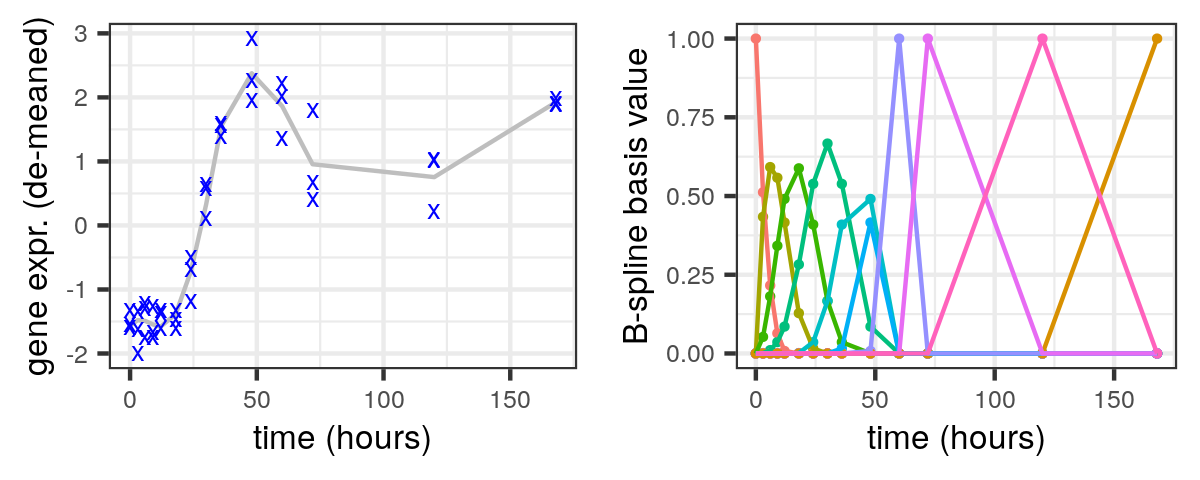
\includegraphics[width=0.980\linewidth,height=0.392\linewidth]{figure/example_genes-1} 

}

\caption[(Left) An example gene and its expression over time.
     (Right) The cubic B-spline with 7 degrees of freedom]{(Left) An example gene and its expression over time.
     (Right) The cubic B-spline with 7 degrees of freedom. }\label{fig:example_genes}
\end{figure}


\end{knitrout}
%






\begin{knitrout}
\definecolor{shadecolor}{rgb}{0.969, 0.969, 0.969}\color{fgcolor}\begin{figure}[!h]

{\centering 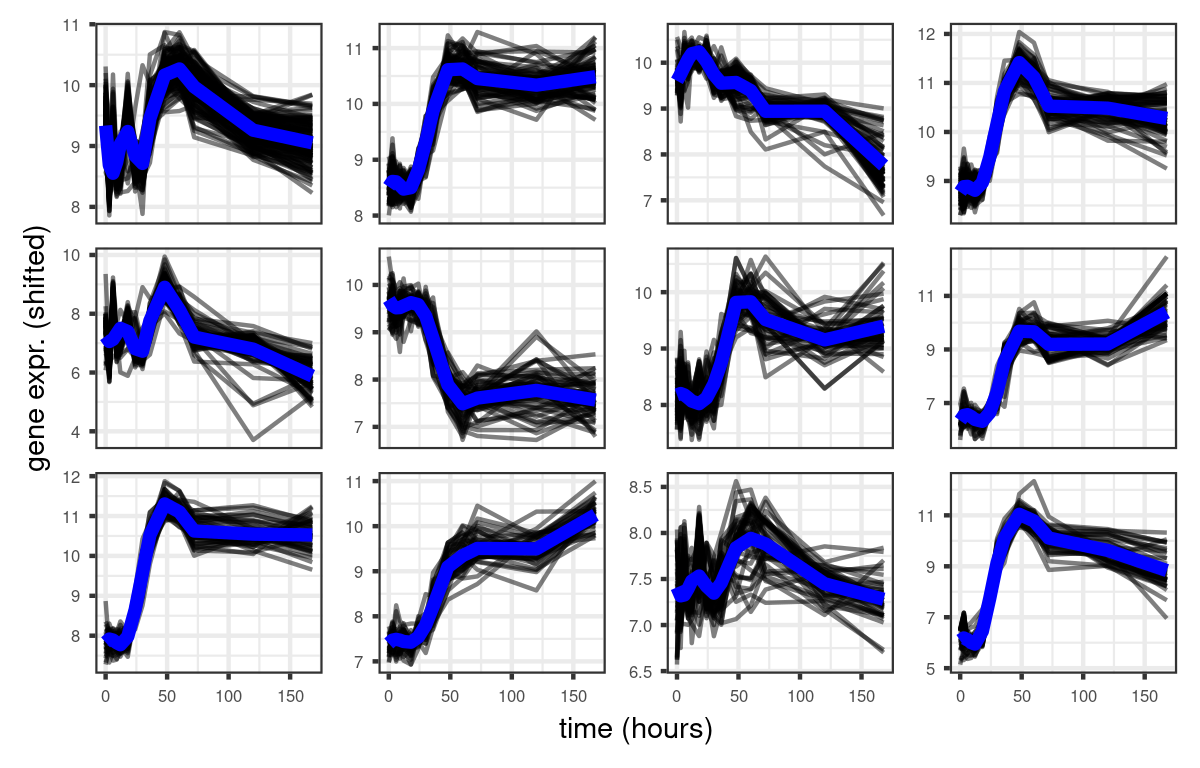
\includegraphics[width=0.980\linewidth,height=0.627\linewidth]{figure/gene_centroids-1} 

}

\caption[In blue, inferred centroids from the twelve most occupied clusters.
    In grey, gene expressions averaged over replicates and
    shifted by their inferred intercepts]{In blue, inferred centroids from the twelve most occupied clusters.
    In grey, gene expressions averaged over replicates and
    shifted by their inferred intercepts. }\label{fig:gene_centroids}
\end{figure}


\end{knitrout}







\begin{knitrout}
\definecolor{shadecolor}{rgb}{0.969, 0.969, 0.969}\color{fgcolor}\begin{figure}[!h]

{\centering 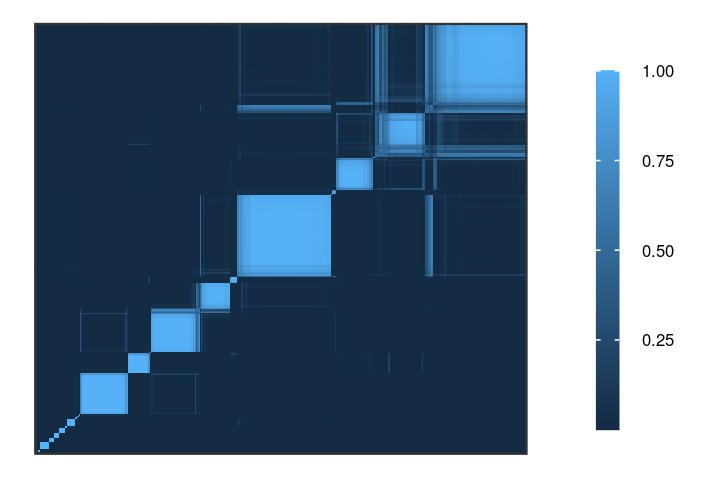
\includegraphics[width=0.588\linewidth,height=0.400\linewidth]{figure/gene_initial_coclustering-1} 

}

\caption[The inferred co-clustering of gene expressions at $\alpha = 3.$ ]{The inferred co-clustering of gene expressions at $\alpha = 3.$ }\label{fig:gene_initial_coclustering}
\end{figure}


\end{knitrout}










\begin{knitrout}
\definecolor{shadecolor}{rgb}{0.969, 0.969, 0.969}\color{fgcolor}\begin{figure}[!h]

{\centering 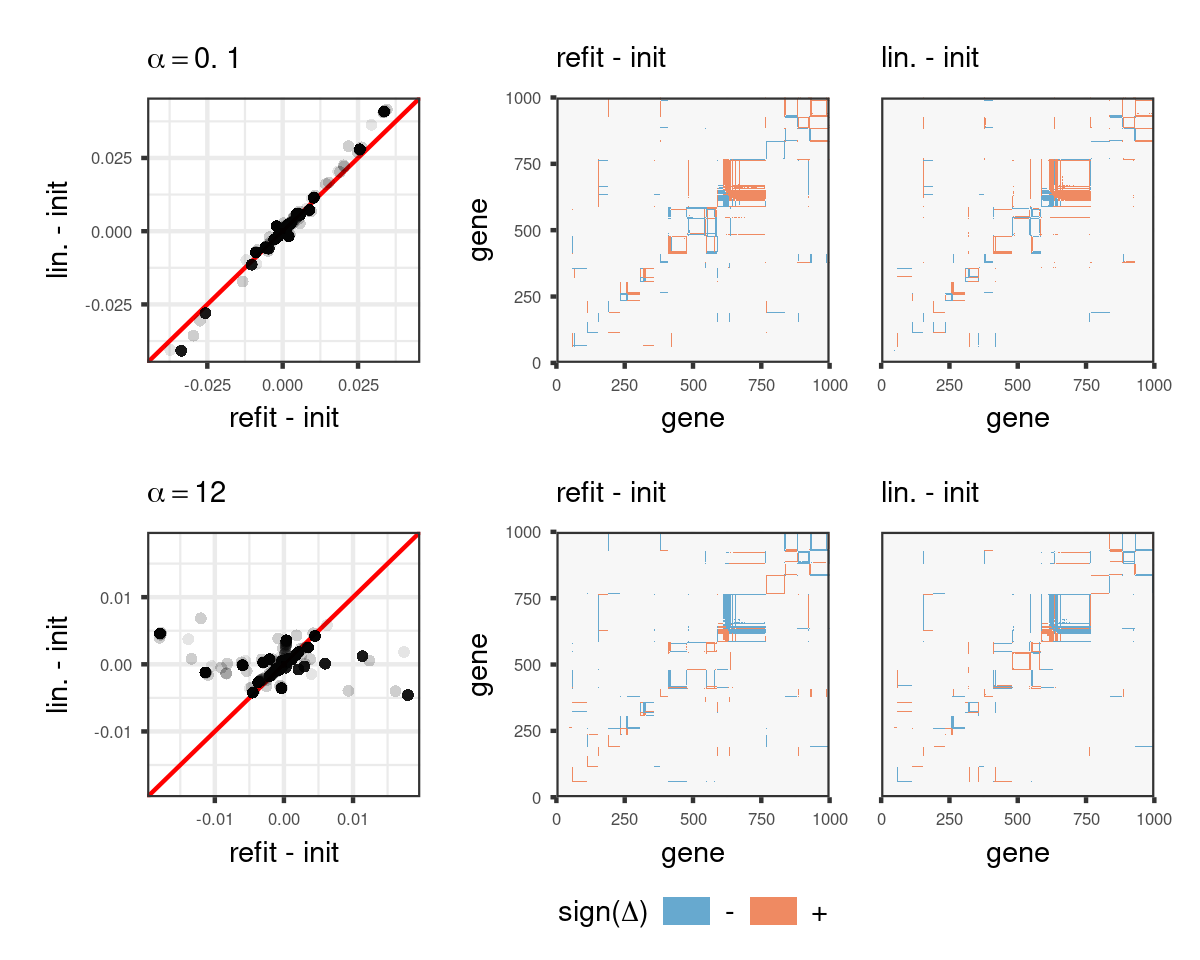
\includegraphics[width=0.980\linewidth,height=0.784\linewidth]{figure/gene_alpha_coclustering-1} 

}

\caption[Changes in the co-clustering matrix at alpha = 1 (top row)
     and alpha = 11 (bottom row),
     relative to the co-clustering matrix at alpha = 3.
     The left column plots differences predicted by the
     linear approximation against differences from a model refit.
     Each point represents an entry of the co-coclustering matrix.
     The middle and right columns display
     changes in the co-clustering matrix as obtained by the
     linear approximation and the model refit, respectively]{Changes in the co-clustering matrix at alpha = 1 (top row)
     and alpha = 11 (bottom row),
     relative to the co-clustering matrix at alpha = 3.
     The left column plots differences predicted by the
     linear approximation against differences from a model refit.
     Each point represents an entry of the co-coclustering matrix.
     The middle and right columns display
     changes in the co-clustering matrix as obtained by the
     linear approximation and the model refit, respectively.}\label{fig:gene_alpha_coclustering}
\end{figure}


\end{knitrout}





\begin{knitrout}
\definecolor{shadecolor}{rgb}{0.969, 0.969, 0.969}\color{fgcolor}\begin{figure}[!h]

{\centering 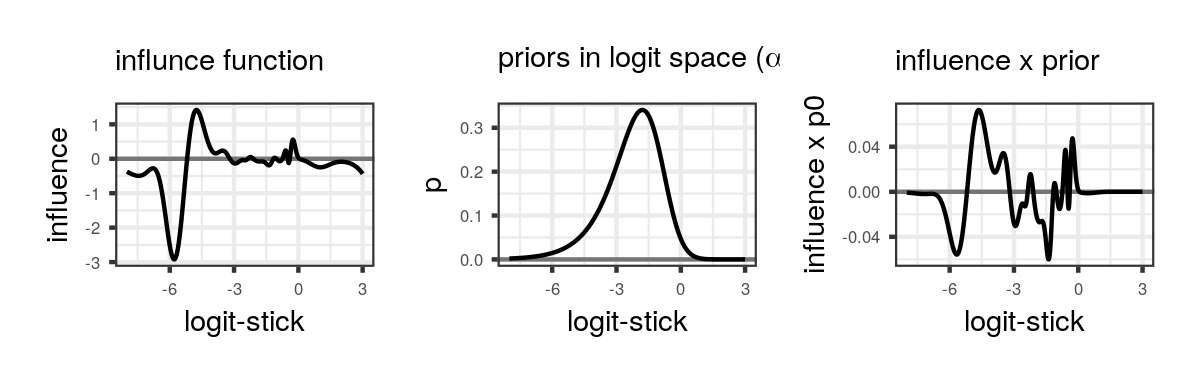
\includegraphics[width=0.980\linewidth,height=0.314\linewidth]{figure/gene_alpha_coclustering_influence-1} 

}

\caption[The influence function of $g_{ev}$, the sum of the eigenvalues of the coclustering Laplacian matrix]{The influence function of $g_{ev}$, the sum of the eigenvalues of the coclustering Laplacian matrix. }\label{fig:gene_alpha_coclustering_influence}
\end{figure}


\end{knitrout}





\begin{knitrout}
\definecolor{shadecolor}{rgb}{0.969, 0.969, 0.969}\color{fgcolor}\begin{figure}[!h]

{\centering 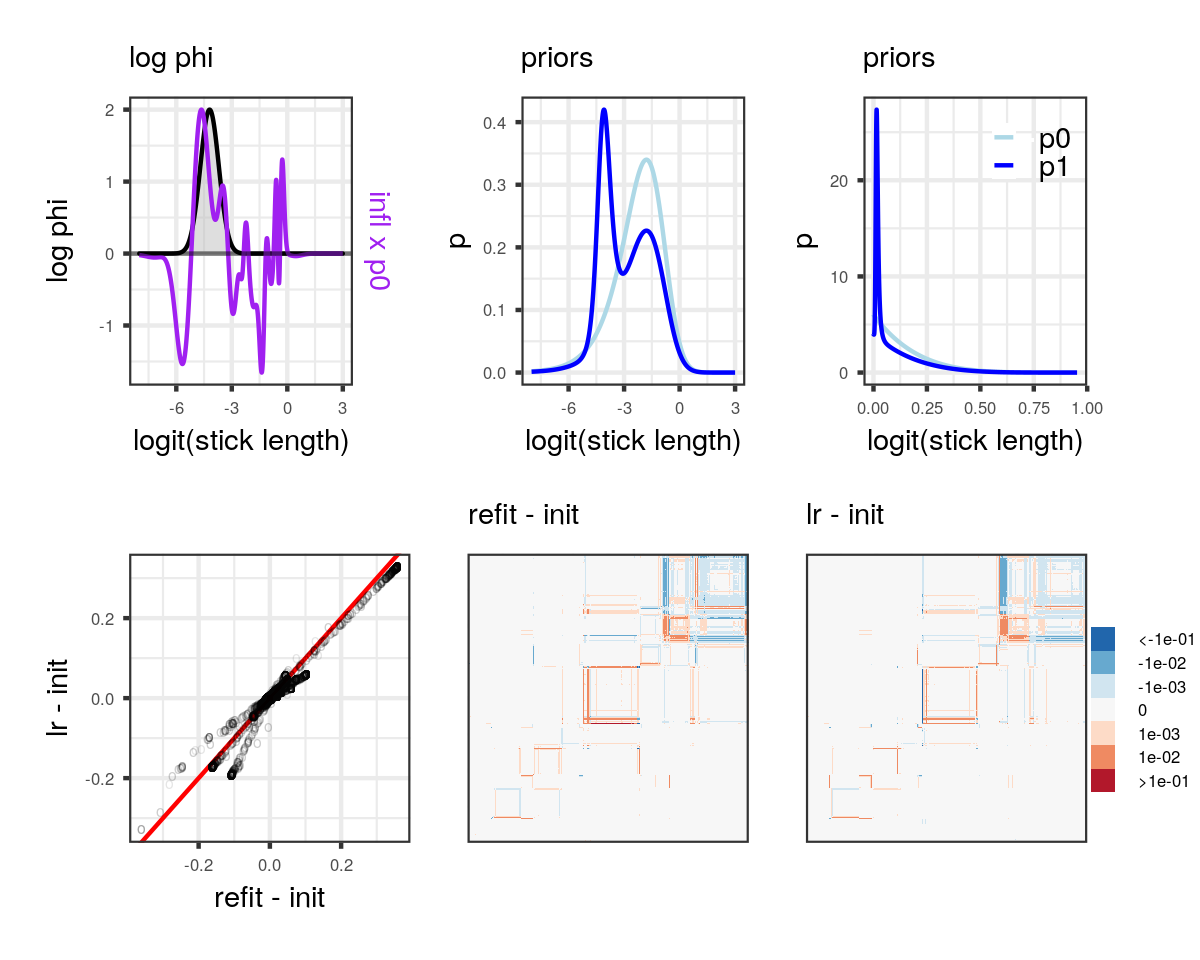
\includegraphics[width=0.980\linewidth,height=0.784\linewidth]{figure/gene_fpert_coclustering-1} 

}

\caption[Effect on the co-clustering matrix after a functional perturbation.
     log-phi (top left, in grey) is set to a Gaussian p.d.f]{Effect on the co-clustering matrix after a functional perturbation.
     log-phi (top left, in grey) is set to a Gaussian p.d.f. centered at mu = -4.2, and scaled to have L-infinity norm equal to two.
    The chosen log-phi roughly corresponds to a positive bump in the influence function of $g_{ev}$.}\label{fig:gene_fpert_coclustering}
\end{figure}


\end{knitrout}



\begin{knitrout}
\definecolor{shadecolor}{rgb}{0.969, 0.969, 0.969}\color{fgcolor}\begin{figure}[!h]

{\centering 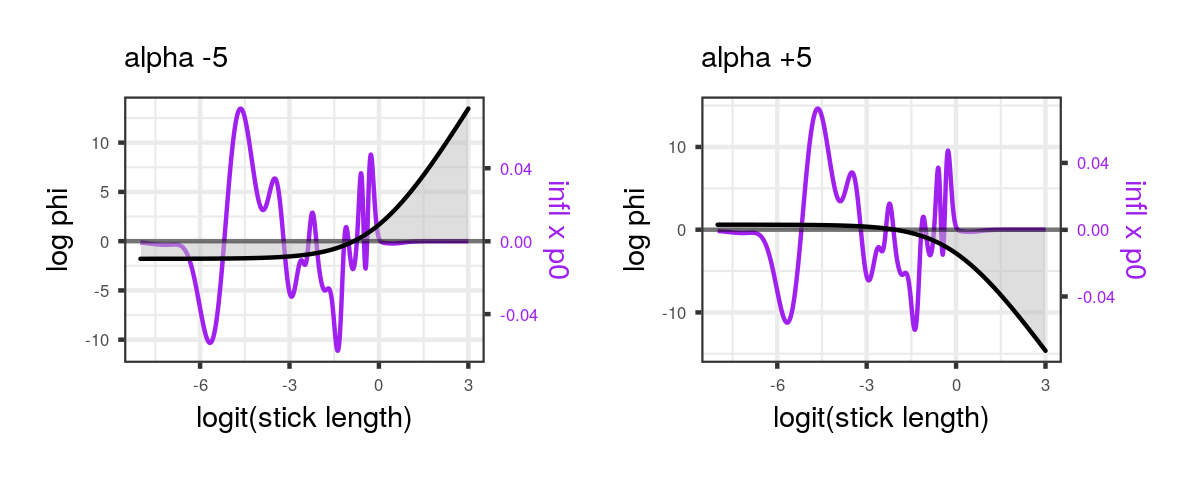
\includegraphics[width=0.980\linewidth,height=0.392\linewidth]{figure/alpha_pert_logphi-1} 

}

\caption[The log multiplicative perturbation $\log \phi$ corresponding to decreasing the $\alpha$ parameter by five (left) or increasing the $\alpha$ parameter by five (right)]{The log multiplicative perturbation $\log \phi$ corresponding to decreasing the $\alpha$ parameter by five (left) or increasing the $\alpha$ parameter by five (right). }\label{fig:alpha_pert_logphi}
\end{figure}


\end{knitrout}
